% ----------------------------------------------------------------
% Report Class (This is a LaTeX2e document)  *********************
% ----------------------------------------------------------------
% Dissertation Template

\documentclass[11pt,oneside]{book}
% \usepackage[margin=1.2in]{geometry}
\usepackage[toc,page]{appendix}
\usepackage{graphicx}
%\usepackage{natbib}
\usepackage{lipsum}
\usepackage{caption}
\usepackage[numbers]{natbib}

%\documentclass[12pt,a4paper]{report}

\usepackage[lmargin=0.5cm,tmargin=0cm,rmargin=1cm,bmargin=0cm]{geometry}
\usepackage{mathptmx}

\begin{document}
\setcounter{tocdepth}{0} 
\renewcommand\labelitemi{---}

\frontmatter

\begin{titlepage}
\begin{center}
{\LARGE University of Sheffield}\\[1.5cm]
\linespread{1.2}\Large {\bfseries EEE339}\\[2cm]
\linespread{1}

\includegraphics[width=9cm]{images/logo.png}\\[1.5cm]

\linespread{1.2}\Large {\bfseries Digital Signal Processing Coursework}\\[1cm]
{\Large Mohammed Ayman Shaikh}\\[1cm]
\large A report submitted in fulfillment of the module\\EEE339 Digital Engineering\\[0.3cm] 
\textit{in the}\\[0.3cm]
School of Electronic and Electrical Engineering\\[2cm]
\today
\end{center}

\end{titlepage}


\linespread{1.5}

% Fonts -- the following two packages give you Times Roman in LaTex
%\usepackage{txfonts}


\pagenumbering{arabic}


\chapter{Introduction}
In this coursework, digital filters will be implemented in MATLAB to remove noise from 
Electrocardiogram (ECG) signals. The file \textbf{ECGData1.mat} will be used for the purposes of this coursework. The diagnosis for this data set was premature ventricular contraction (PVC), in a 69 year-old male.
\chapter{Original and Noisy ECG Signals}
Below, two plots can be seen. 
\\The first plot is the original ECG signal, and the second is the same signal, but with added noise.
\begin{center}
%\centering
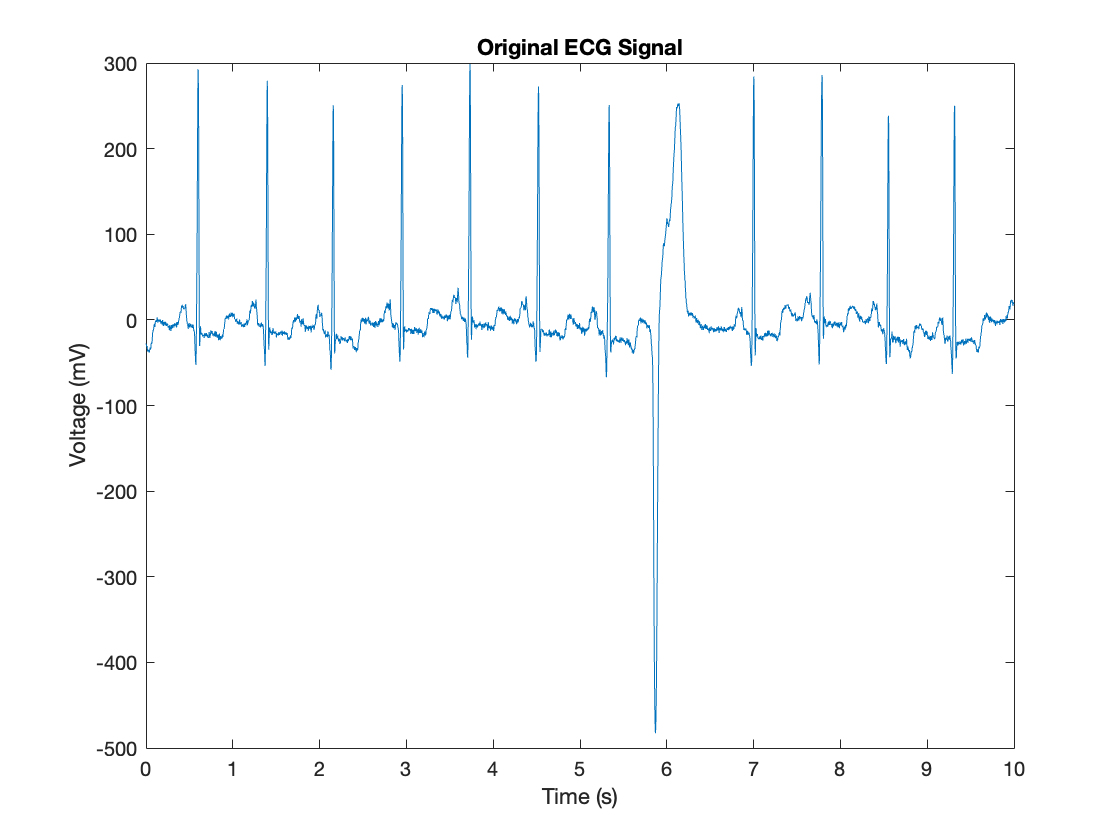
\includegraphics[width=14cm]{graphics/orig.png}
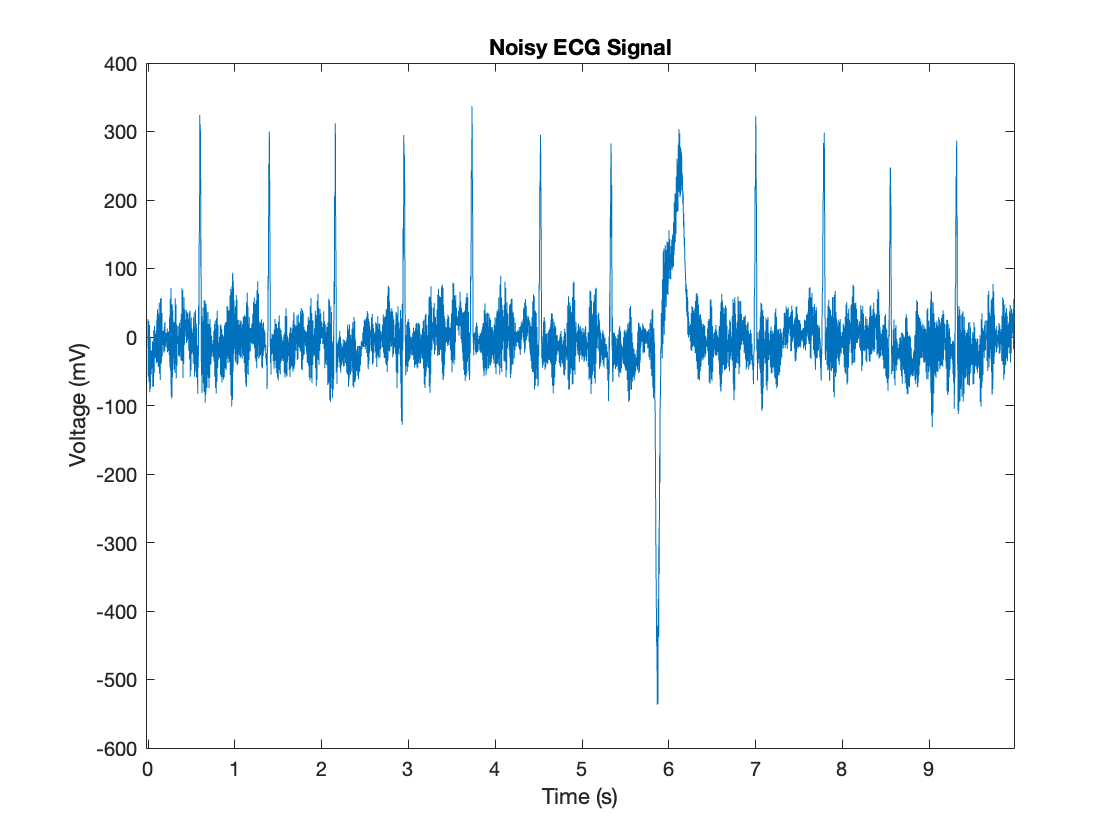
\includegraphics[width=14cm]{graphics/noisy.png}
\end{center}
\chapter{Heart Rate Calculation}
Heart rate can be calculated using the number of QRS Complexes in the ECG signals and the timeframe of the signal recorded.
Since 12 QRS Complexes can be seen in both signals and the timeframe of the recorded signals is 10 seconds, we use this formula to calculate the heart rate in beats per minute (bpm):
\begin{center}
    $\textit{Heart Rate} = \frac{\textit{Number of QRS Complexes}}{\textit{Timeframe}} \times 60 = \frac{12}{10} \times 60 = 72$ bpm
\end{center}
\chapter{Fast Fourier Transform}
On the below plot, the FFT of the noisy ECG signal can be seen. Two abnormaltiies can be seen: the mains hum at 60Hz, due to the data being recorded in the USA, as well as the high-frequency spikes between 120-140Hz, likely due to muscle contractions or other biological phemomena.
\\These two abnormaltiies can be removed from the plot by using a low pass filter around 55Hz. The equivalent normalised frequency is 0.306, calculated using the following formula:
\begin{center}
    $\textit{Normalised Frequency} = \frac{\textit{2 * Cutoff Frequency}}{\textit{Sampling Frequency }} = \frac{2 * 55}{360} = \frac{110}{360} = 0.306$
    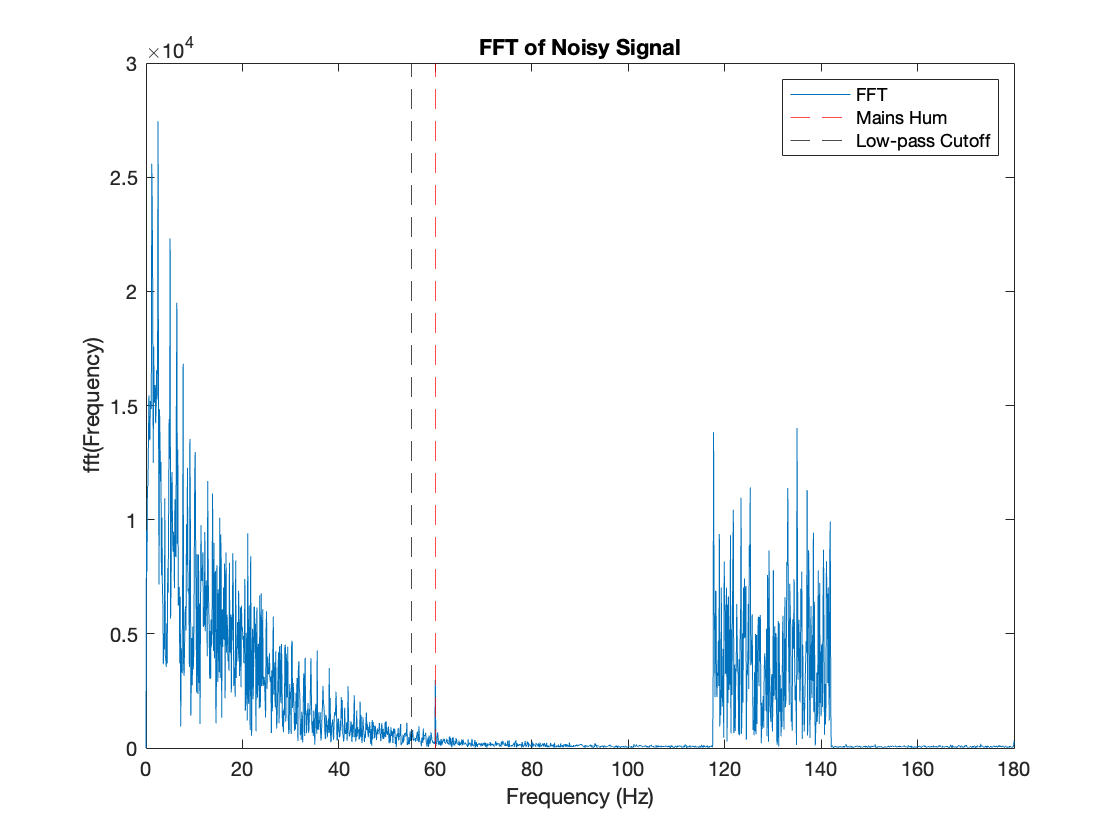
\includegraphics[width=16cm]{graphics/noisy_fft.png}
\end{center}
\chapter{IIR and FIR Filtering}
Fifth order and 55Hz cutoff was chosen for the filters, since it leads to the best frequency attenuation.
\begin{center}
    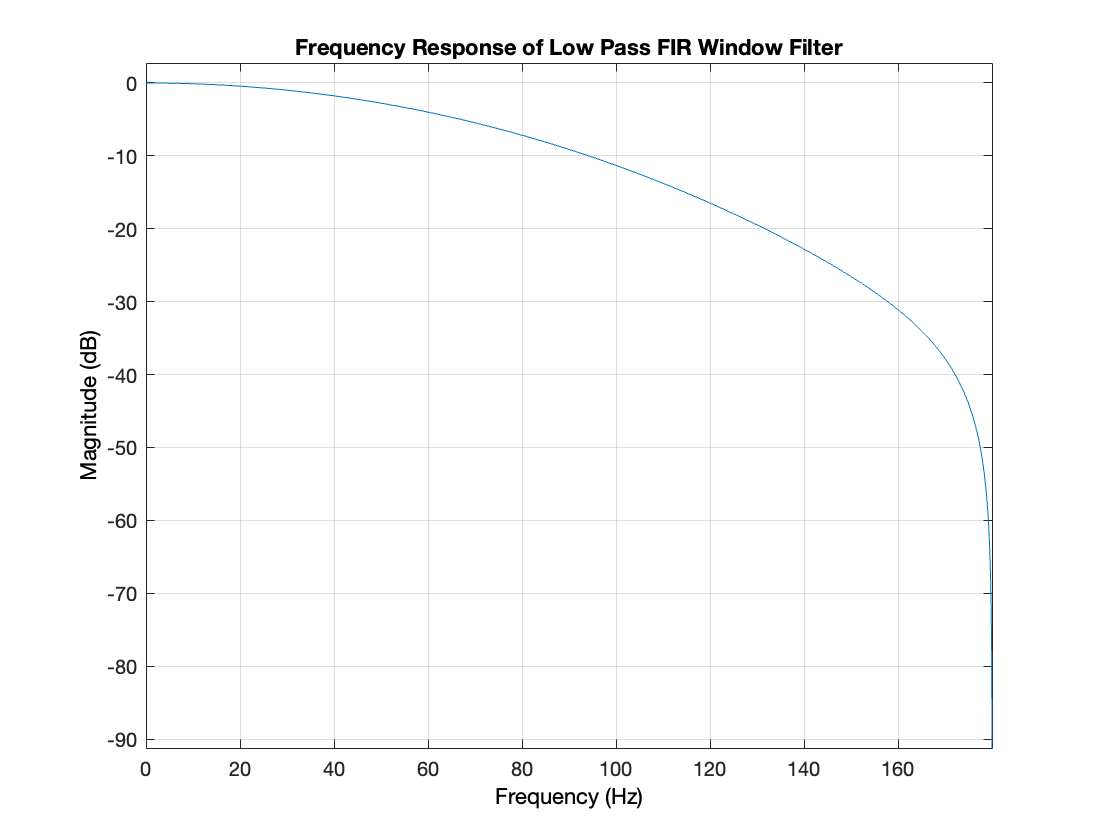
\includegraphics[width=14cm]{graphics/fir_o5.png}
    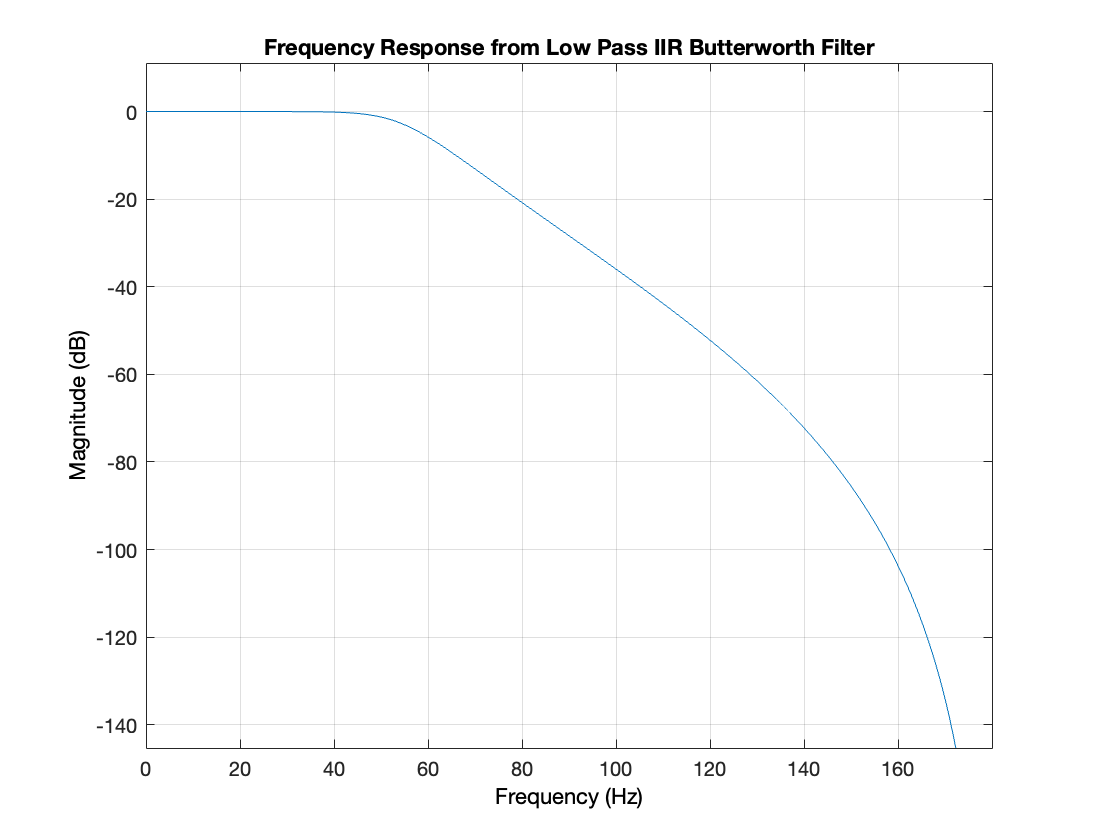
\includegraphics[width=14cm]{graphics/iir_o5.png}
    
\end{center}
\chapter{Original, Noisy and Filtered Signals}
The below plot shows the original ECG signal, the two filtered ECG signals, and the noisy signal. 
The FIR filters smoothed the output more and IIR filters reduced noise better. 
\\[0.1cm]
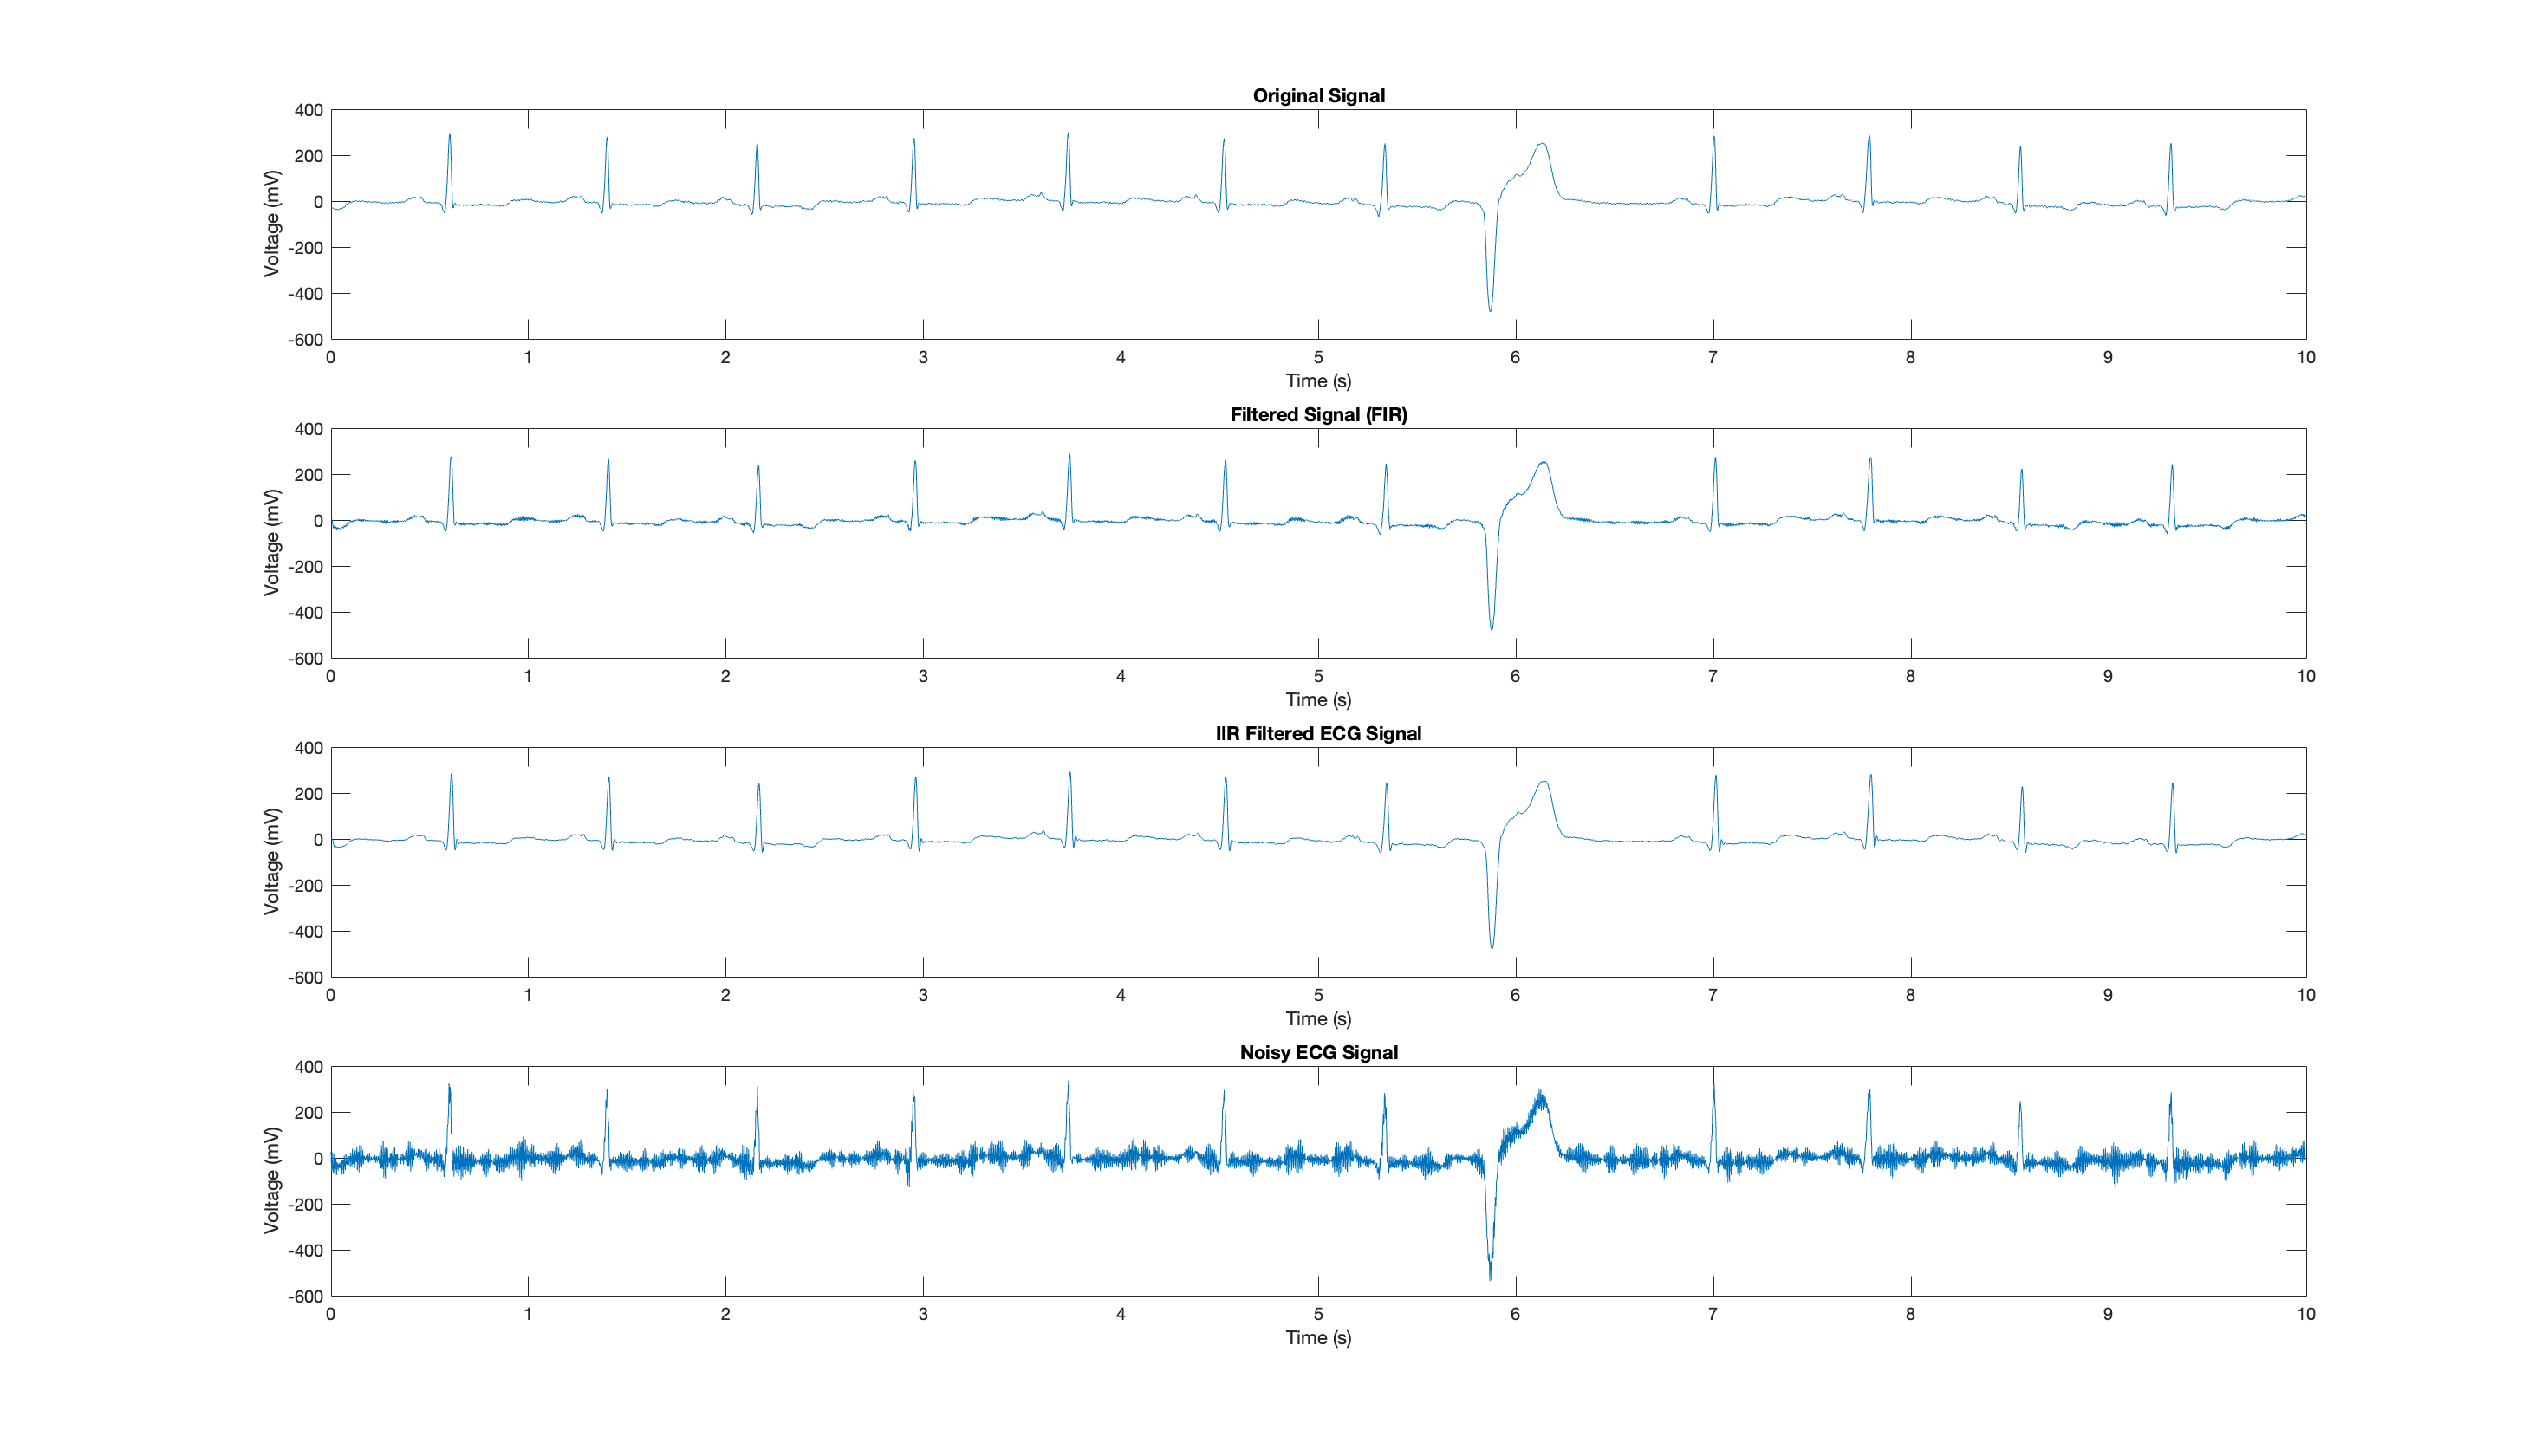
\includegraphics[width=23cm]{graphics/four_signals.png}

\chapter{Improving the Filter Design}
In hindsight, it might have been a better idea to use multiple filters to target the mains hum and the high-frequency spikes separately. This would have led to a better filter design, and a better filtered signal.
\\We could use raise the cutoff frequency of the low pass filter to around 100Hz, and then use a notch filter to remove the mains hum at 60Hz.\\[0.1cm]
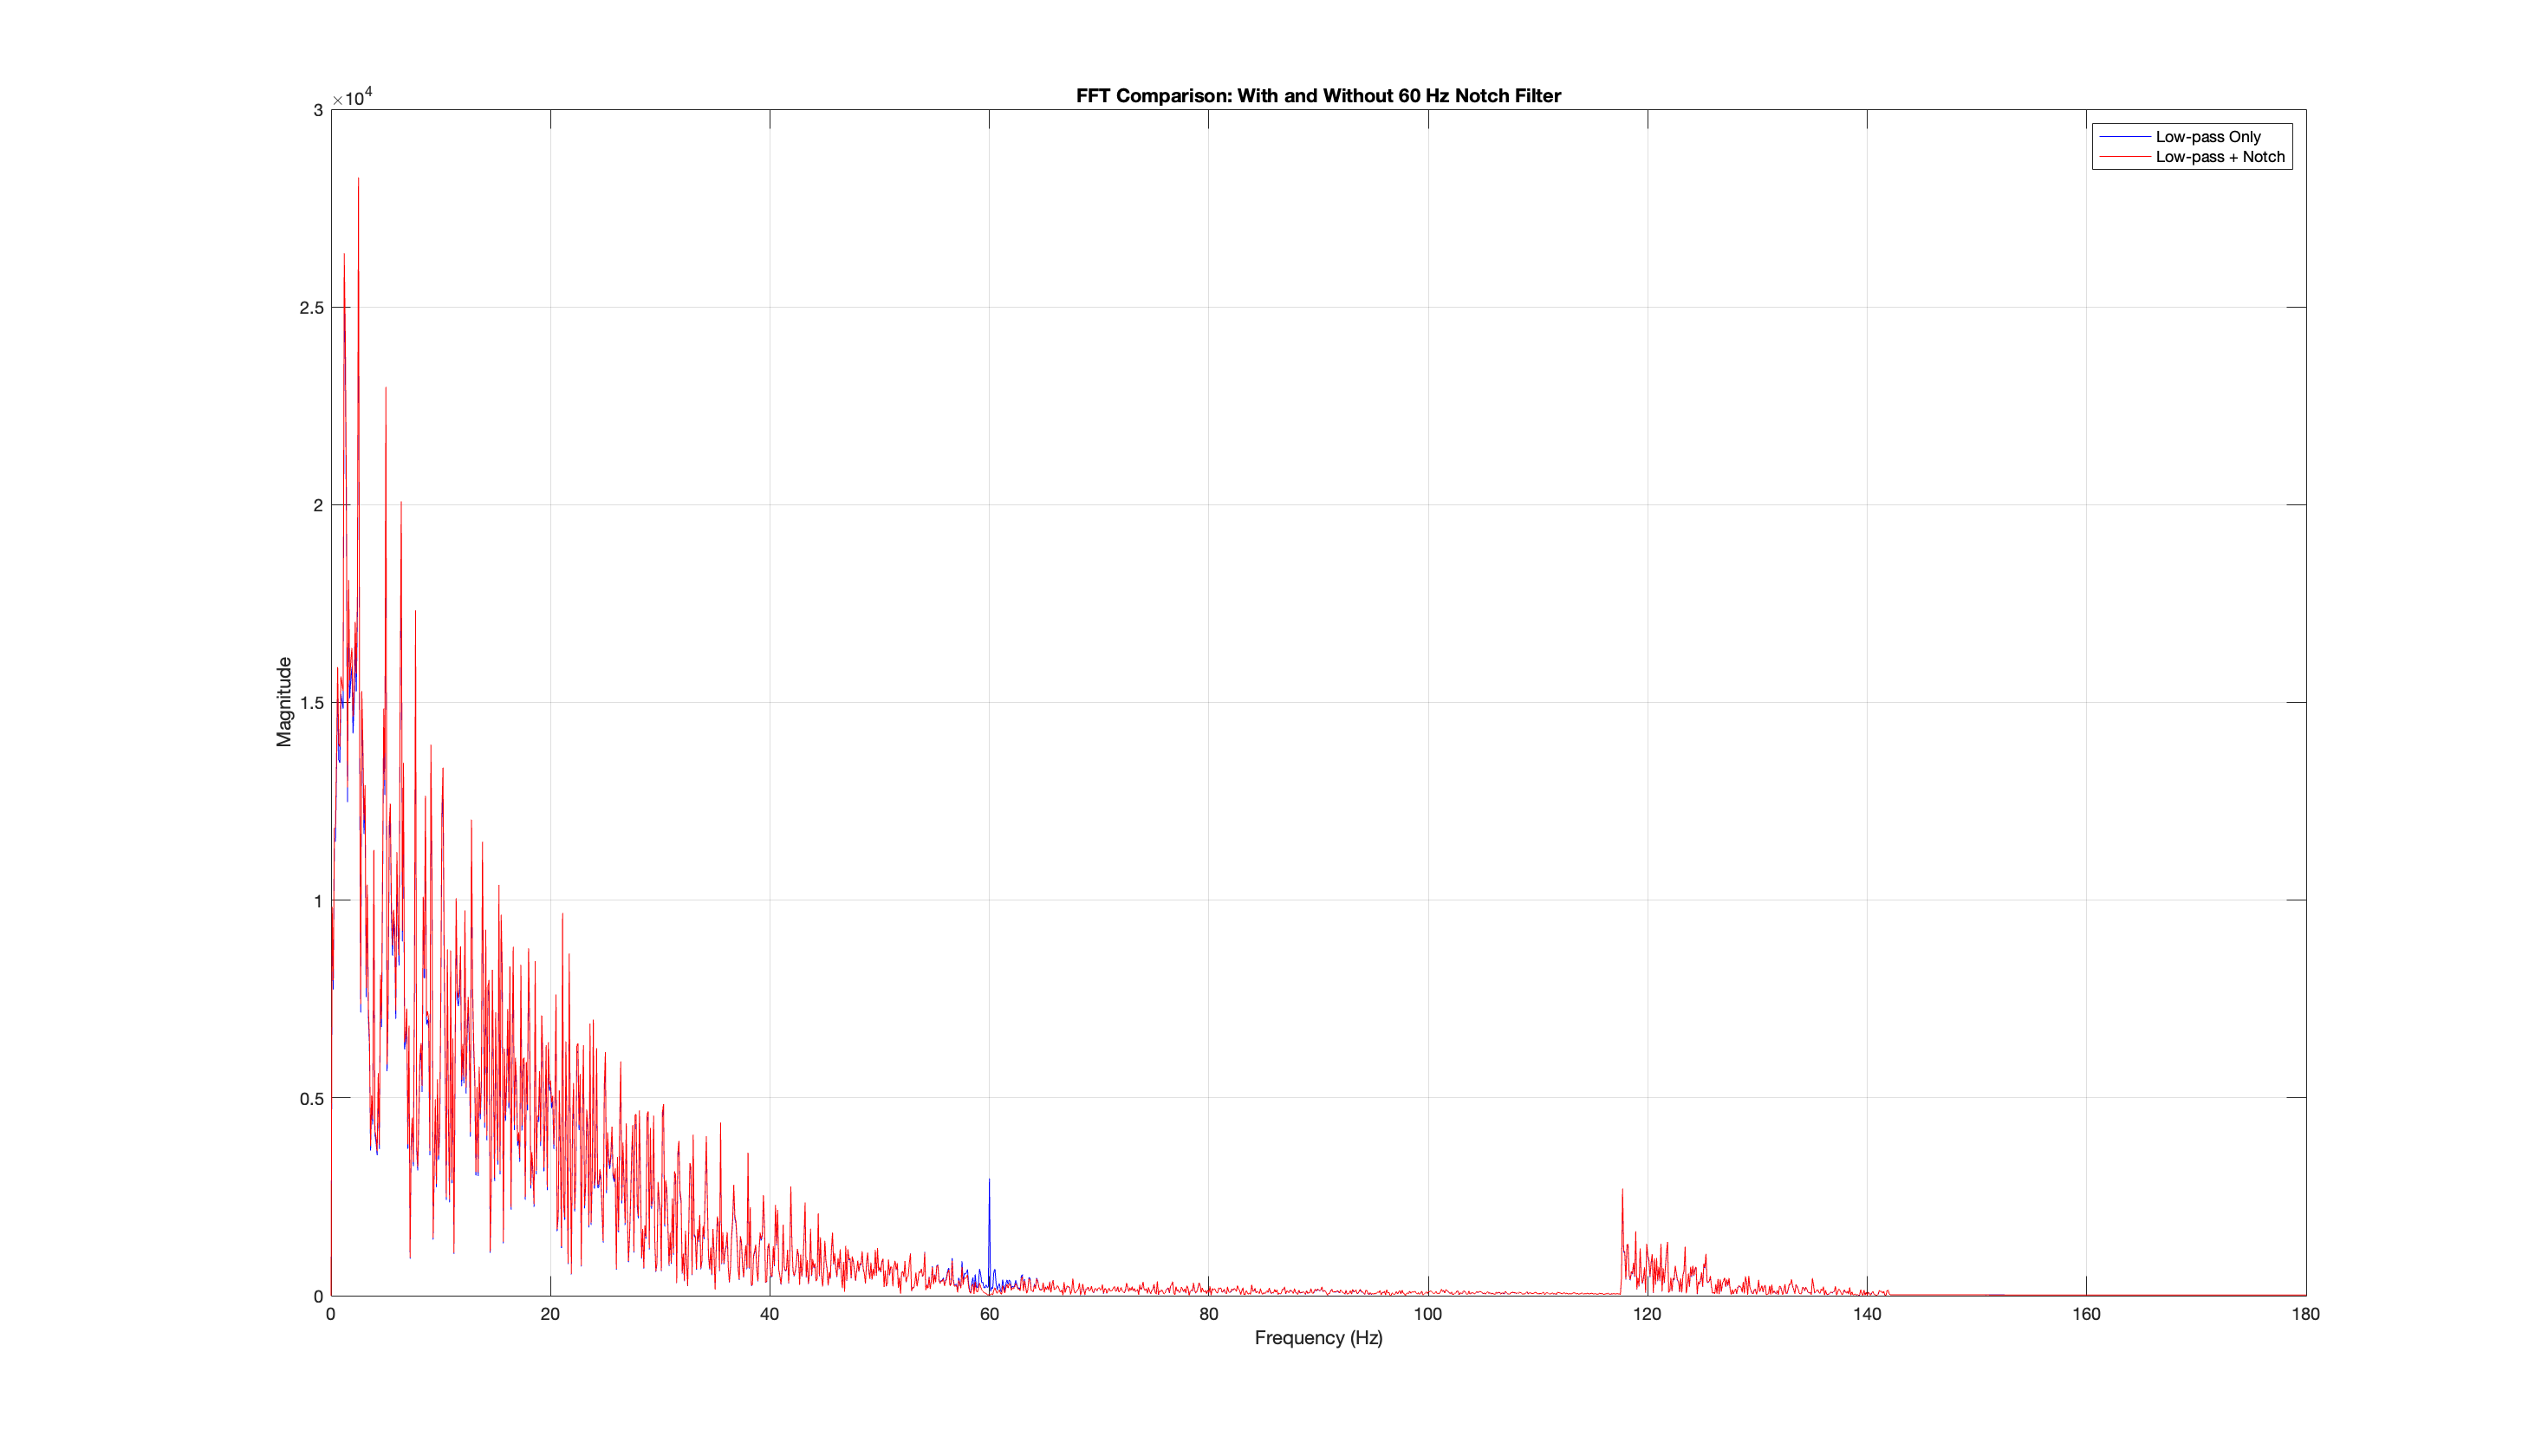
\includegraphics[width=20cm]{graphics/notched_fft.png}\\
In this plot, the FFT of the filtered signal, with a higher cutoff of 100Hz, can be seen. The notched filter can be seen in red, showing that the notch works to effectively attenuate the mains hum.
\\The high frequency spikes have also been mostly attenuated by the higher cutoff of the low pass filter.\\[0.1cm]
\end{document}
% ----------------------------------------------------------------

% End of Report Class (This is a LaTeX2e document) ***************